\documentclass{article}
\usepackage[margin=1in]{geometry}
\usepackage{amsmath,amsthm,amssymb}
\usepackage{bbm,enumerate,mathtools}
\usepackage{tikz,pgfplots}
\usepackage{chessboard}
\usepackage[hidelinks]{hyperref}
\usepackage{multicol} % Problem 35

\newenvironment{question}{\begin{trivlist}\item[\textbf{Question.}]}{\end{trivlist}}
\newenvironment{note}{\begin{trivlist}\item[\textbf{Note.}]}{\end{trivlist}}
\newenvironment{references}{\begin{trivlist}\item[\textbf{References.}]}{\end{trivlist}}
\newenvironment{related}{\begin{trivlist}\item[\textbf{Related.}]\end{trivlist}\begin{enumerate}}{\end{enumerate}}


\begin{document}
\rating{3}{3}
Consider all of the ``essentially distinct'' ways of starting with two points on the plane, and then with a straightedge/compass drawing $n$ lines/circles. This forms a graded poset, where the chains the poset correspond to an algorithm for constructing that diagram.

\begin{figure}[ht!]
  \[
    \begin{tikzpicture}
      \node[draw] (A1) at (0,0) {
        \begin{tikzpicture}
          \fill (0,0) circle (0.1);
          \fill (1,0) circle (0.1);
        \end{tikzpicture}
      };
      \node[draw] (B1) at (-2,2) {
        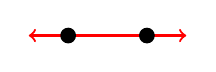
\begin{tikzpicture}
          \draw[thick, red, <->] (-0.5,0) -- (1.5,0);
          \fill (0,0) circle (0.1);
          \fill (1,0) circle (0.1);
        \end{tikzpicture}
      };
      \node[draw] (B2) at (2,2) {
        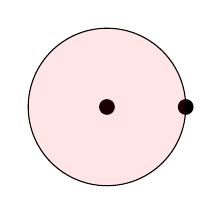
\begin{tikzpicture}
          \fill (0,0) circle (0.1);
          \fill (1,0) circle (0.1);
          \draw[fill=red, fill opacity=0.1] (0,0) circle (1);
        \end{tikzpicture}
      };
      \node[draw] (C1) at (-2,5) {
        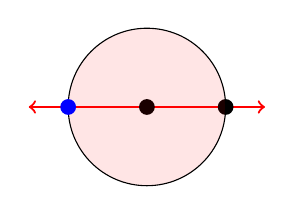
\begin{tikzpicture}
          \draw[thick, red, <->] (-1.5,0) -- (1.5,0);
          \fill (0,0) circle (0.1);
          \fill (1,0) circle (0.1);
          \draw[fill=red, fill opacity=0.1] (0,0) circle (1);
          \fill[blue] (-1,0) circle (0.1);
        \end{tikzpicture}
      };
      \node[draw] (C2) at (4,5) {
        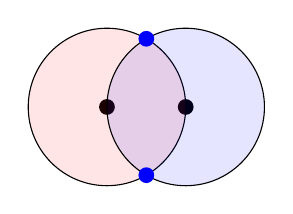
\begin{tikzpicture}
          \fill (0,0) circle (0.1);
          \fill (1,0) circle (0.1);
          \draw[fill=red, fill opacity=0.1] (0,0) circle (1);
          \draw[fill=blue, fill opacity=0.1] (1,0) circle (1);
          \fill[blue] (1/2,{sqrt(3)/2}) circle (0.1);
          \fill[blue] (1/2,{-sqrt(3)/2}) circle (0.1);
        \end{tikzpicture}
      };
      \node[draw] (D1) at (-3,9) {
        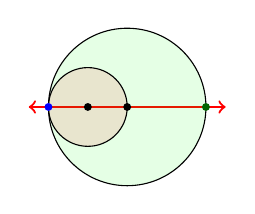
\begin{tikzpicture}[scale=0.5]
          \draw[<->, thick, red] (-1.5,0) -- (3.5,0);
          \draw[fill=green, fill opacity=0.1] (1,0) circle (2);
          \draw[fill=red, fill opacity=0.1] (0,0) circle (1);
          \fill (0,0) circle (0.1);
          \fill (1,0) circle (0.1);
          \fill[blue] (-1,0) circle (0.1);
          \fill[green!40!black] (3,0) circle (0.1);
        \end{tikzpicture}
      };
      \node[draw] (D2) at (-0.25,9) {
        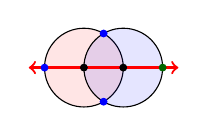
\begin{tikzpicture}[scale=0.5]
          \draw[fill=red, fill opacity=0.1] (0,0) circle (1);
          \draw[fill=blue, fill opacity=0.1] (1,0) circle (1);
          \draw[<->, thick, red] (-1.4,0)--(2.4,0);
          \fill (0,0) circle (0.1);
          \fill (1,0) circle (0.1);
          \fill[blue] (1/2,{sqrt(3)/2}) circle (0.1);
          \fill[blue] (1/2,{-sqrt(3)/2}) circle (0.1);
          \fill[green!40!black] (2,0) circle (0.1);
          \fill[blue] (-1,0) circle (0.1);
        \end{tikzpicture}
      };
      \node[draw] (D3) at (2,9) {
        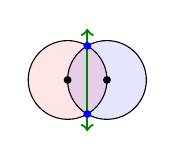
\begin{tikzpicture}[scale=0.5]
          \draw[fill=red, fill opacity=0.1] (0,0) circle (1);
          \draw[fill=blue, fill opacity=0.1] (1,0) circle (1);
          \draw[<->, thick, green!50!black] (1/2,-1.3)--(1/2,1.3);
          \fill (0,0) circle (0.1);
          \fill (1,0) circle (0.1);
          \fill[blue] (1/2,{sqrt(3)/2}) circle (0.1);
          \fill[blue] (1/2,{-sqrt(3)/2}) circle (0.1);
        \end{tikzpicture}
      };
      \node[draw] (D4) at (4,9) {
        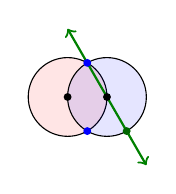
\begin{tikzpicture}[scale=0.5]
          \draw[fill=red, fill opacity=0.1] (0,0) circle (1);
          \draw[fill=blue, fill opacity=0.1] (1,0) circle (1);
          \draw[<->, thick, green!50!black] (0,{sqrt(3)})--(2,{-sqrt(3)});
          \fill[green!40!black] (1.5,{-sqrt(3)/2}) circle (0.1);
          \fill (0,0) circle (0.1);
          \fill (1,0) circle (0.1);
          \fill[blue] (1/2,{sqrt(3)/2}) circle (0.1);
          \fill[blue] (1/2,{-sqrt(3)/2}) circle (0.1);
        \end{tikzpicture}
      };
      \node[draw] (D5) at (6,9) {
        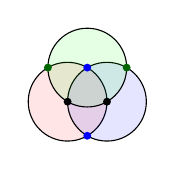
\begin{tikzpicture}[scale=0.5]
          \draw[fill=red, fill opacity=0.1] (0,0) circle (1);
          \draw[fill=blue, fill opacity=0.1] (1,0) circle (1);
          \draw[fill=green, fill opacity=0.1] (1/2,{sqrt(3)/2}) circle (1);
          \fill (0,0) circle (0.1);
          \fill (1,0) circle (0.1);
          \fill[blue] (1/2,{sqrt(3)/2}) circle (0.1);
          \fill[blue] (1/2,{-sqrt(3)/2}) circle (0.1);
          \fill[green!40!black] (1.5,{sqrt(3)/2}) circle (0.1);
          \fill[green!40!black] (-0.5,{sqrt(3)/2}) circle (0.1);
        \end{tikzpicture}
      };
      \node[draw] (D6) at (8,9) {
        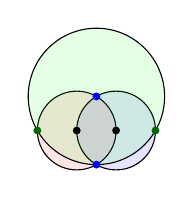
\begin{tikzpicture}[scale=0.5]
          \draw[fill=red, fill opacity=0.1] (0,0) circle (1);
          \draw[fill=blue, fill opacity=0.1] (1,0) circle (1);
          \draw[fill=green, fill opacity=0.1] (1/2,{sqrt(3)/2}) circle ({sqrt(3)});
          \fill (0,0) circle (0.1);
          \fill (1,0) circle (0.1);
          \fill[green!40!black] (2,0) circle (0.1);
          \fill[green!40!black] (-1,0) circle (0.1);
          \fill[blue] (1/2,{sqrt(3)/2}) circle (0.1);
          \fill[blue] (1/2,{-sqrt(3)/2}) circle (0.1);
        \end{tikzpicture}
      };
      \draw
        (A1) -- (B1)
        (A1) -- (B2)
        (B1) -- (C1)
        (B2) -- (C1)
        (B2) -- (C2)
        (C1) -- (D1)
        (C1) -- (D2)
        (C2) -- (D2)
        (C2) -- (D3)
        (C2) -- (D4)
        (C2) -- (D5)
        (C2) -- (D6)
      ;
    \end{tikzpicture}
  \]
  \caption{
    A ruler/straightedge poset.
  }
\end{figure}

\begin{question}
  Consider the ranked poset of diagrams. How many diagrams are at rank $n$?
\end{question}

\begin{related}
  \item What is the greatest/least number of regions for an element at rank $n$?
  \item What is the greatest/least number of points for an element at rank $n$?
  \item What is the number of distinct distances over all of rank $n$? (e.g. rank $2$ has distances of $1$, $2$, and $\sqrt{3}$. Rank $3$ has distances of $1$, $2$, $3$, $4$, and $\sqrt{3}$.)
  \item Is this poset Sperner?
\end{related}

\begin{note}
  I suspect that it's easy to prove by induction that the least number of points for an element at rank $n$ is $n + 2$, by continually making the biggest possible circle centered at the rightmost point.
\end{note}
\begin{references}
  \item OEIS: Yuda Chen's \href{https://oeis.org/A352903}{A352903} and my \href{https://oeis.org/A383744}{A383744}.
  \item MSE: Joel David Hamkins, ``\href{https://math.stackexchange.com/q/3377988/121988}{What is the next number on the constructibility sequence?}''
\end{references}
\end{document}
